\chapter{Literature Review}
\label{ch:review}

\section{Use of Neural Networks to Accelerate Error-\\Tolerant Applications}

In \cite{Esmaeilzadeh2012}, and algorithmic transformation, called the Parrot transformation, is proposed. It is a way of selecting regions of imperative code and training a neural network to mimic it, then a specialized hardware accelerator, a neural processing unit, is utilized to run the transformed code.

Figure \ref{fig:NPU_flow} shows the full workflow to utilize the algorithmic transformation technique. The programmer needs to annotate the code to indicate the compiler which parts to optimize and transform to a neural network. Then the compiler trains a neural network utilizing input data given by the user as well as some parameters to define the hyperparameters and architecture of the neural network. After that, code is generated that can run in an architecture that can configure the NPU to run the approximate parts of the program. Speedups ranging from 0.8x to 11.1x were achieved, as well as energy reductions ranging from 1.1 to 21.1. The experiments were run using the MARSSx86 simulator.

\begin{figure}[thbp]
	\centering
	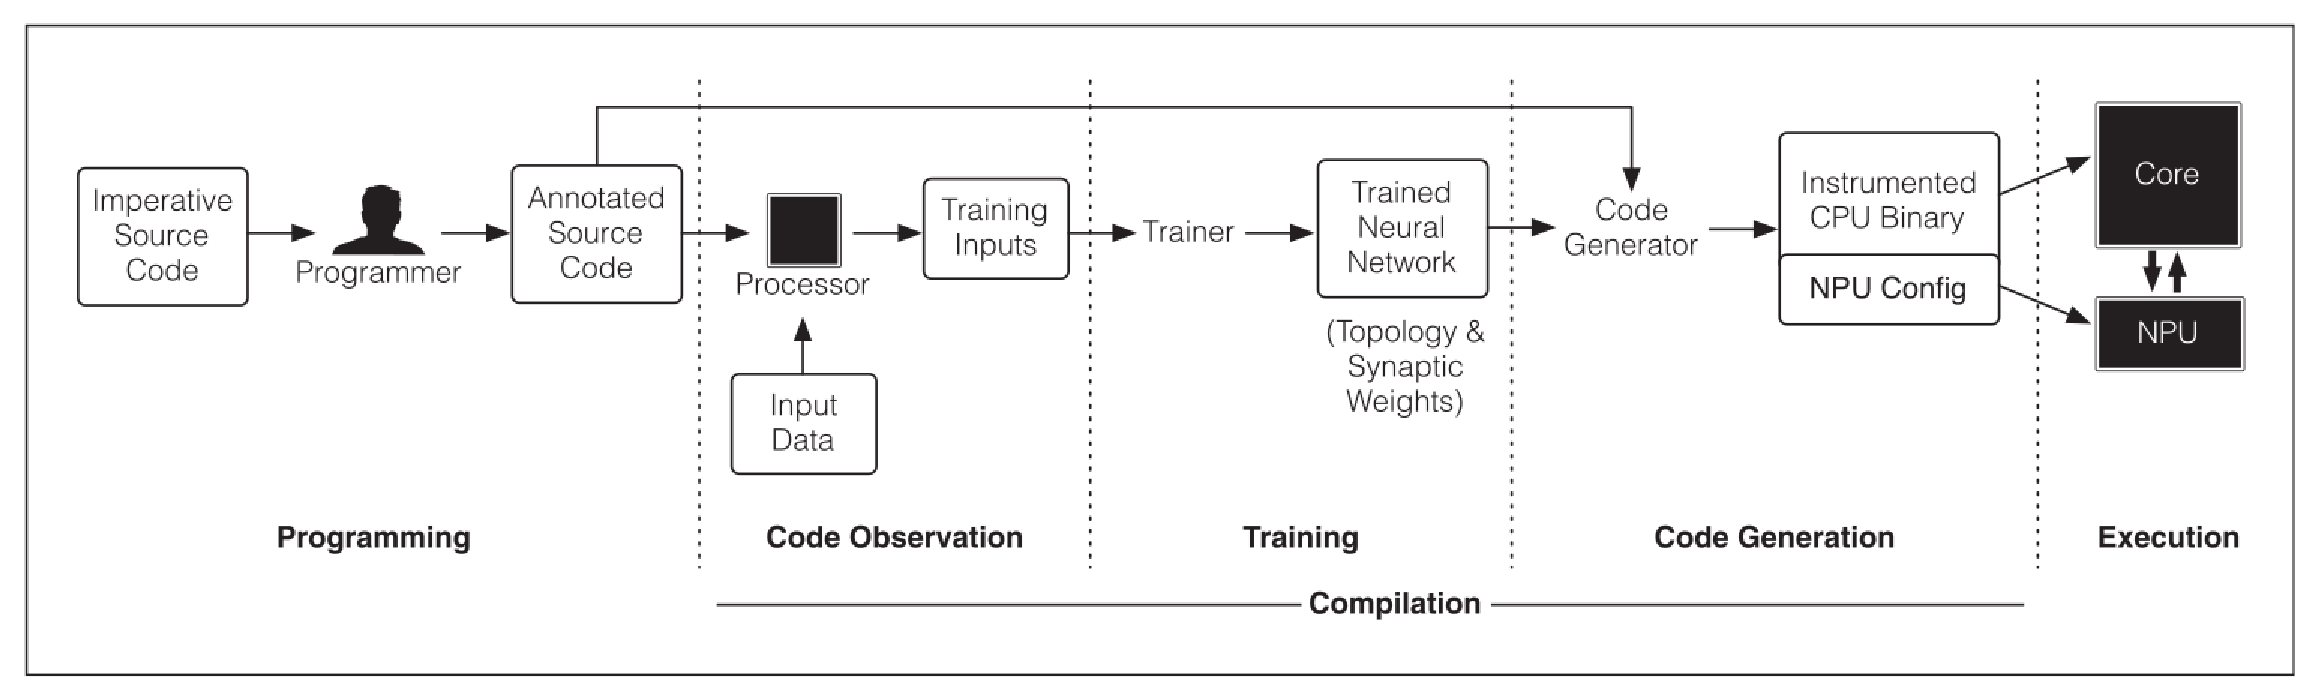
\includegraphics[scale=0.3]{NPU_flow}
	\caption[Work flow for approximate computing using NPUs.]{Work flow for approximate computing using NPUs \cite{Esmaeilzadeh2012}.}
	\label{fig:NPU_flow}
\end{figure}

In \cite{Moreau2015a} and \cite{Moreau2015} a novel method to do approximate transformations to code is proposed. Specifically, in \cite{Moreau2015a}, a high-level overview of both the software and hardware solutions is presented. ACCEPT is a compiler framework for approximate programs. It extends the C and C++ syntax to incorporate an APPROX keyword that can be used to annotate data types. Based on the annotations it applies program transformations only for the approximate data. It identifies regions of code that are safe to approximate. Then it executes the program with test cases and records input-output data to train a neural network that mimics the code using the back-propagation algorithm. Finally, it generates a binary that replaces the original code with invocations to the NPU.

In \cite{Moreau2015}, the SNAPP NPU is presented, it is designed to work with the ACCEPT compiler framework. It evaluates multi-layer perceptron (MPL) neural networks, using an array of Processing Units (PUs). Each PU consists of a chain of Processing Elements (PEs), a sigmoid unit and local memories. A PE consists of a multiply-and-add module implemented on a DSP slice. The sigmoid unit applies the neural network’s activation function to outputs from the PE chain. Speedups from 1.46x to 38.12x were achieved. Energy savings were on the 0.54x to 20.04x range. The platform used was the ZYNQ ZC702, which includes a 2-core ARM Cortex-A9 and a Xilinx Artix-7 FPGA (TSMC 28nm).

\section{Optimization of Neural Networks Using Approximate Computing Techniques}

This section explores the work that has been done to optimize inference on neural networks using approximate computing and other techniques. This can be done either in software, hardware or both.

In \cite{Venkataramani2015} a new technique is proposed that transforms a neural network into an approximate version of it that can run in a specialized hardware designed for it. They demonstrate that by utilizing this technique energy efficiency can be improved up to 1.92 times with little loss ($<$ 0.5\%).

Spiking neural networks are a new generation of neural networks that more closely mimic natural neural networks. In \cite{Sen2017}, the authors propose AxSNN, a new effort to apply approximate computing to improve the energy efficiency of SNNs. AxSNN achieved energy improvements of up to 3.62X using a specialized approximate accelerator.

In \cite{Peng2018} a novel method of training approximate neural networks is proposed. This method deploys two neural networks, an approximator and a predictor. These work together to guarantee the quality of the results. These optimized networks improve training time, have better energy efficiency and have less error than the non-approximate equivalent.

Pruning and quantization are techniques that can be helpful to improve performance and energy efficiency in neural networks. In \cite{Hanif2018} several case studies are presented which leverage these software level techniques as well as the use of approximate multipliers implemented in hardware to perform weighted sum operations.

In \cite{Sarwar2018} two algorithm level approximations are explored: lowering the network complexity and pruning. The first one consists of simply reducing the number of layers and/or neurons per layer with the objective to achieve improvements in energy efficiency without hurting the accuracy too much. Similarly, pruning removes certain connections in the neural network and reduces the complexity. In the same paper the authors also propose hardware level approximations: an approximate multiplier for neural computation and a voltage-scaled approximate memory for on-chip synaptic storage.

\section{Neural Network Accelerators}

The use of algorithmic transformations clearly show improvements to speed and power consumption, this is great but it can't be efficiently done in the real world unless those computations can be offloaded to an accelerator that can execute neural networks fast and with low power. This section will describe the Cambricon and Myriad accelerators, which are available commercially.

In \cite{Liu2016}, Cambricon, an instruction set architecture for neural networks is presented. The Cambricon ISA focuses on three areas: data-level parallelism, customized vector/matrix instructions and using on-chip scratchpad memory (instead of vector registers) to provide flexible width for each data access. It provides four types of instructions: computational (arithmetic and others for matrix/vector/scalars), variable-size data transfer (load/store/move for matrix/vector/scalars), logical (compare/logic for vector/scalar) and control (jump, conditional branch).

Using the Cambricon ISA, the Cambricon-X NPU is described at \cite{Zhang2016}. Cambricon-X's architecture consists on a control processor (CP), a buffer controller (BC), two neural buffers (NBin and NBout) to store input and output neurons, a direct memory access module (DMA) and a computation unit (CU) which contains multiple processing elements (PEs). The BC selects needed neurons for each PE from local neuron buffers based on the loaded instructions which are decoded by the CP, and transfers those neurons to PEs for efficient local computation.

The Movidius Myriad I is the first generation visual processing unit (VPU) designed by Movidius. It is designed for power-efficient computation. It has eight highly specialized cores focused in SIMD (single instruction multiple data) processing called SHAVEs (streaming hybrid architecture vector engines). The SHAVE processors are vector VLIW (very long instruction word) processors designed to crunch complex vision and imaging algorithms at high performance and low power. Each SHAVE core has assigned 128 Kbyte slices of SRAM memory, for a total of 1 MB. This memory is arranged in a CMX (connection matrix) topology. It also has 128 Kbytes of L2 cache which can be partitioned into independent caches. The chip runs at a top frequency of 200 MHz, with the memory clocked at 133 MHz \cite{Ionica2015}.

The Myriad 2 is the second generation of VPUs designed by Movidius. It now features twelve vector processors (SHAVEs) and double the memory (2 MB). The SHAVE processors are a new and improved version (3.0). The L2 cache is also doubled, getting it to a total of 256 Kbytes. The SoC now includes a new SIPP (streaming image processing pipeline) computational imaging hardware accelerators. The SHAVE cores themselves offer a 5x performance increase, now clocked at 600 MHz. On top of that the SIPP hardware accelerators can provide 15-25x additional performance \cite{Moloney2014}.

\begin{figure}[thbp]
	\centering
	\includegraphics[scale=0.35]{myriad_x}
	\caption[Myriad X VPU Architecture.]{Myriad X VPU Architecture \cite{myriad_vpus}}
	\label{fig:myriad_x}
\end{figure}

The Myriad X is the third generation of Movidius VPUs. The SHAVE processors count is increased to sixteen and the internal memory to 2.5 MB. It now also includes a dedicated deep neural network processing unit: the Neural Compute Engine, which can improve computations up to 10x \cite{myriadx}. The operating frequency received a bump to 700 MHz. Figure \ref{fig:myriad_x} shows a diagram of the Myriad X architecture. Table \ref{tab:myriad_vpus} compares the hardware specifications of the Myriad 2 and Myriad X VPUs. The most viable way of obtaining the Myriad VPUs is through the Intel Neural Compute Stick. The first generation used the Myriad 2 VPU and the latest iteration uses the newer Myriad X VPU. This is simple USB3 stick that plugs into any device and allows for offloading of neural network computations at a very low power. \cite{ncs2}

\begin{table}[thbp]
	\centering
	\caption[Movidius Myriad Family VPUs.]{Movidius Myriad Family VPUs \cite{myriad_vpus}}
	\label{tab:myriad_vpus}
	\resizebox{\textwidth}{!}{%
		\begin{tabular}{|c|c|c|}
			\hline
			& \textbf{Myriad 2}                                                                                             & \textbf{Myriad X}                                                                                                                   \\ \hline
			Compute Capacity             & \textgreater{}1 TOPS                                                                                 & \textgreater{}4 TOPS                                                                                                       \\ \hline
			Vector Processors            & 12x SHAVE Processors                                                                                 & 16x SHAVE Processors                                                                                                       \\ \hline
			CPUs                         & \begin{tabular}[c]{@{}c@{}}2x LEON4 cores\\ (RISC; SPARC V8)\end{tabular}                            & \begin{tabular}[c]{@{}c@{}}2x LEON4 cores\\ (RISC; SPARC V8)\end{tabular}                                                  \\ \hline
			On-chip Accelerators         & $\sim$20 image/vision processing accelerators                                                        & \begin{tabular}[c]{@{}c@{}}20+ image/vision processing accelerators\\ Neural Compute Engine (DNN accelerator)\end{tabular} \\ \hline
			Neural Network Capability    & \begin{tabular}[c]{@{}c@{}}1st Gen DNN Support\\ (Up to 100 GFLOPS)\end{tabular}                     & \begin{tabular}[c]{@{}c@{}}Neural Compute Engine\\ (Up to 1 TOPS)\end{tabular}                                             \\ \hline
			On-chip Memory and Bandwidth & \begin{tabular}[c]{@{}c@{}}2 MB\\ (400GB/sec)\end{tabular}                                           & \begin{tabular}[c]{@{}c@{}}2.5 MB\\ (450GB/sec)\end{tabular}                                                               \\ \hline
			DRAM Support                 & \begin{tabular}[c]{@{}c@{}}Max: 8Gb\\ LPDDR2 (533MHz, 32-bit)\\ LPDDR3 (933MHz, 32-bit)\end{tabular} & \begin{tabular}[c]{@{}c@{}}Max: 16Gb\\ LPDDR4 (1600MHz, 32-bit)\end{tabular}                                               \\ \hline
			DRAM Configurations          & \begin{tabular}[c]{@{}c@{}}1Gbit LPDDR2 (MA215X)	\\ 4Gbit LPDDR3 (MA245X)\end{tabular}               & \begin{tabular}[c]{@{}c@{}}No in-package memory (MA2085)		\\ 4Gbit LPDDR4 (MA2485)\end{tabular}                            \\ \hline
			Encoder/Codec                & VGA, 720p, 1080p, H.264 (software encoder)                                                           & \begin{tabular}[c]{@{}c@{}}M/JPEG 4K at 60Hz encoder\\ H.264/H.265 4K at 30Hz encoder\end{tabular}                         \\ \hline
			Key Interfaces               & \begin{tabular}[c]{@{}c@{}}12x MIPI lanes (DPHY 1.1)\\ USB 3\\ SPI\\ I2S\\ SD\\ 1GbE\end{tabular}    & \begin{tabular}[c]{@{}c@{}}16x MIPI lanes (PHY 1.2)\\ USB 3.1\\ Quad SPI\\ I2S\\ 2x SD\\ 10GbE\\ PCIe 3.0\end{tabular}     \\ \hline
			Process                      & 28nm HPC+/HPC/HPM (TSMC)                                                                             & 16nm FFC (TSMC)                                                                                                            \\ \hline
			Package                      & \begin{tabular}[c]{@{}c@{}}6.5mm x 6.5 mm (MA215X)\\ 8mm x 9.5 mm (MA245X)\end{tabular}              & 8.1mm x 8.8mm (MA2085, MA2485)                                                                                             \\ \hline
		\end{tabular}%
	}
\end{table}

\section{Review of Applications Using OpenVINO and Myriad VPUs}

To be able to program a neural processing unit such as the Myriad Family of devices, a programming framework needs to be provided to be able to access the hardware functions of the accelerator. Intel provides the OpenVINO toolkit to be able to program the Myriad accelerators. This section will review the work that has been done using the OpenVINO toolkit and the Movidius Myriad VPUs.

In \cite{Tiwari2019}, neural networks for image classification are deployed to the first generation of Intel Neural Compute Stick (NCS), which uses the Myriad 2 VPU. The results are compared against a Core i5-5200 CPU. The inference time in the CPU are lower (0.027 - 0.039 seconds) compared to what the NCS can provide (0.238 - 0.290). The advantage of the NCS is the power consumption, it uses 1.2 Watts while the CPU uses up to 69. This means that the performance per Watt is much better in the NCS (2.837 - 3.501 inferences/second/Watt) than in the CPU (0.371 - 0.536).

An analysis of the acceleration of neural networks inference on Intel processors is done in \cite{Andriyanov2020}. This study shows that using OpenVINO can significantly improve performance in Intel hardware. It compares a classical implementation with TensorFlow against an optimize version using OpenVINO. The results show that the OpenVINO version are significantly faster, with gains ranging from 88.07x up to 175.23x, with an average gain of 126.449x.

Low power devices with limited computing capacity can benefit substantially when offloading neural network computations to an external accelerator. This is what is demonstrated in \cite{Benelli2019}. A comparison is made between running inference in a Raspberry Pi 3 using the Caffe framework versus using the NCS running the model optimized with OpenVINO. The results show improvements in inference time and in energy per inference of up to 50\% with a loss of accuracy below 0.4\%.

In \cite{Castro-Zunti2020} a license plate segmentation and recognition system is tested. The baseline performance is 59 ms per inference, this is using TensorFlow on an Intel Xeon CPU with 12 cores. When the model is optimized using OpenVINO, the inference time is reduced to 14 ms. Transferring the application to a low-cost, low-power embedded system using the Raspberry Pi 3 and the Intel Neural Stick 2 means that the inference time is increased to 66 ms, which is only 7 ms more than the original un-optimized version running in the CPU.

One popular solution for accelerating neural networks is using FPGAs to offload the heavy processing. In \cite{Marantos2018}, the Xilinx Zynq-7000 was programmed, using HLS (High Level Synthesis), to run the SVM (Support Vector Machines) classifier. The same application was implemented using the Myriad 2 VPU and the results show that the power consumption is 80\% lower at the cost of doubling the execution time.

In \cite{Xu2018}, an application that uses 3D CNNs is deployed to three different platforms: an Nvidia Titan X GPU, an Intel i7-5930K CPU and the Movidius NCS. The performance in the GPU is highly superior, with an inference time of 0.5 ms, the NCS follows with 11 ms and lastly the CPU takes 13 ms. The efficiency of the NCS shines in this application, since the inference per seconds per watt is 75.75 vs 0.8 and 0.81 in the GPU and CPU respectively.

A lung nodule detection application was tested in several platforms in \cite{Mathew2019}. The results show a great reduction in inference time when running the application using OpenVINO versus Caffe. In an Intel i7 CPU the time improves from 7.5 seconds in Caffe to 0.2304 with OpenVINO. Even when deploying the application to the low-power NCS2, the inference time is reduced to 0.8142 seconds. The only tested configuration that is faster than OpenVINO is when running Caffe in an Nvidia GTX 1080 GPU.
